\documentclass[12pt]{article}

% Include packages required to compile document:
\usepackage{amsmath} % For mathematical symbols and environments
\usepackage{amsfonts} % For math fonts
\usepackage{amssymb} % For additional symbols
\usepackage{animate} % For gif images
\usepackage{graphicx} % For including images
\usepackage{hyperref} % For hyperlinks
\usepackage{geometry} % For customizing page margins
\usepackage{indentfirst} % Load the indentfirst package

% Page setup
\geometry{margin=1in} % Customize margins if needed

% Title
\title{X Power X: A Journey from Real to Complex}
\author{Patrick Su}

\begin{document}

\maketitle

\begin{abstract}

This report explores the fascinating world of complex exponentiation, starting from the real plane and extending into the complex plane. 
The goal is to delve into the mathematical intricacies of functions like $(-1)^x$ and $x^x$, and how their behaviors change when we consider complex solutions. 
I will also investigate the role of the parameter $k$ in determining the number of revolutions in the complex plane.
Feel free to skip parts that are famailiar to you and enjoy the ride.
\end{abstract}

\section[Math in Section]{The Real Part of the graph $y = x^x$}

We will start with something famailiar: the real part of the function. In real analysis, the domain of the function is often $x>0$ since the function is well defined and obtains real outputs.

For the negative part, things get complicated. For example, the following is real: \[ (-2)^{-2} = \frac{1}{(-2)^2} = \frac{1}{4} \]
But the following is complex: \[(-\frac{1}{2})^{-\frac{1}{2}} = \frac{1}{\sqrt{(-\frac{1}{2})}} = \frac{1}{i\sqrt{2}} = -\frac{i}{\sqrt{2}}\]
Don't worry if you are confused, we will elaborate them in later sections.

Although $0^0$ is consided to be 1 for convenience in some contexts like combinatorics, in the context of this report, we will consider it indeterminate. 
However, we can still find the limit behavior near 0 from the right hand side.
\subsection[Math in Subsection]{The behaviors of the graph as $x \rightarrow 0^{+}$}
Before we do any algebra manipulation, it is worth pointing out that $x^x$ is equivalent to $e^{ln(x^x)}=e^{xln(x)}$ (recall that $a=e^{ln(a)}$). We can then derive the following limit:
\[ \lim_{{x \to 0^+}} x^x = \lim_{{x \to 0^+}} e^{xln(x)} = \lim_{{x \to 0^+}} e^{\frac{ln(x)}{\frac{1}{x}}} 
= e^{\lim_{{x \to 0^+}} \frac{ln(x)}{\frac{1}{x}}} = e^{\lim_{{x \to 0^+}} \frac{\frac{1}{x}}{-\frac{1}{x^2}}}
= e^{\lim_{{x \to 0^+}} -x} = 1\]

\subsection{The critical points}
First, we need to find the values of $x$ where the derivative of the function is equal to zero or undefined. I will provide two different ways to find the derivative of $y=x^x$. 

The first method utilizes the observation that $e^{ln(x^x)}=e^{xln(x)}$. Using the chain rule and the product rule, we have:

\[ y' = \frac{d}{dx}[e^{x \ln(x)}] = e^{x \ln(x)} \cdot \frac{d}{dx}[x \ln(x)] = e^{x \ln(x)} \cdot (\ln(x) + x \cdot \frac{1}{x}) = x^x \cdot (\ln(x) + 1)\]

Another way to differentiate the function is to take natural logarithm of both sides of the equations (like how you solve some differential equations).
\[ \ln(y) = \ln(x^x) \]

Use the properties of logarithms to simplify the right side.
\[ \ln(y) = x \ln(x) \]

Differentiate both sides with respect to $x$.
\[ \frac{d}{dx}[\ln(y)] = \frac{d}{dx}[x \ln(x)] \]

Apply the chain rule on the left side and the product rule on the right side.
\[ \frac{1}{y} \cdot \frac{dy}{dx} = 1 \cdot \ln(x) + x \cdot \frac{1}{x} \]

Simplify the equation, we have 
\[ \frac{dy}{dx} = y \cdot (\ln(x) + 1) = x^x \cdot (\ln(x) + 1) \]

Now we can find the critical points by setting the first derivative to zero and solve for x. Since $0^0$ is indeterminant and all other outputs for $y=x^x$ are nonzero if defined when $x\neq0$, 
the only solution for the equation is when $ln(x) + 1 = 0 \implies x = e^{-1}$. 

\subsection{Concavity}
We can also determine the concavity of the function by completing a second derivative test.
\[ y'' = \frac{d}{dx}[x^x \cdot (\ln(x) + 1)] \]

Apply the product rule and chain rule 
\[ y'' = \frac{d}{dx}[x^x] \cdot (\ln(x) + 1) + x^x \cdot \frac{d}{dx}[\ln(x) + 1] \]

Subsitute the first derivative, we have
\[ y'' = x^x \cdot (\ln(x) + 1) \cdot (\ln(x) + 1) + x^x \cdot \frac{1}{x} \]

Simplify the expression, we have
\[ y'' = x^x \cdot ((\ln(x) + 1)^2 + \frac{1}{x}) \]

For $x>0$, this expression is positive as $x^x$, $(\ln(x) + 1)^2$ and $\frac{1}{x}$ are all positive in this domain. 
This then indicates the function is concave up at $x=e^{-1}$, suggesting that it has a local minimum at this point..
\subsection{Summary}

The function \(y = x^x\) is not defined at \(x = 0\) due to an indeterminate form but we may analyze its limit near $0$ to identify the behavior
(note it does not mean that the expression itself is undefined, but rather that it cannot be uniquely determined by straightforward evaluation)

There is one critical point at \(x = e^{-1}\).

The second derivative test suggests that the function has a local minimum at \(x = e^{-1}\).

With all the derived information from Calculus, we can gain a sense of the key properties of the graph in the real plane. 
Here is the graph ploted by Mathematica for $x>0$:
\begin{figure}[h]
    \centering
    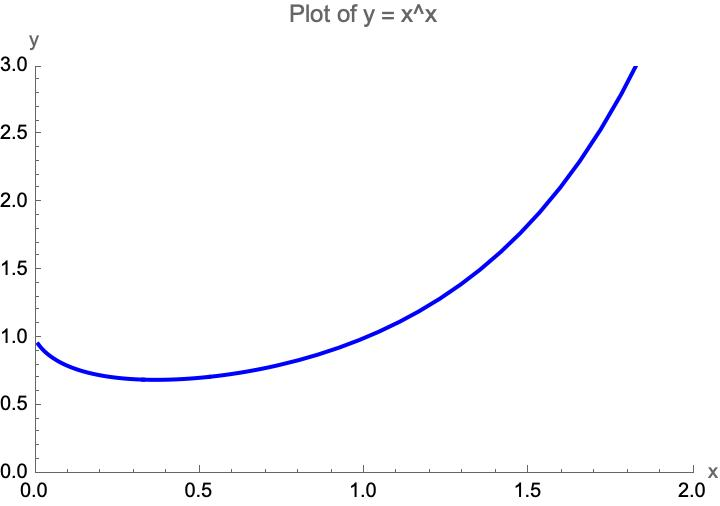
\includegraphics[width=0.5\textwidth]{x-power-x-real.jpeg}
    \label{fig:realPlot}
\end{figure}  
\section{Complex Exponentiation}


\section{Understanding Graphs with Complex Solutions}

\section[Math in Section]{The graph $y = (-1)^x$}

\section[Math in Section]{The graph $y = x^x$}

\section{Miscellaneous}

\end{document}
